\section{Runterschreiben}
\label{sec:rusch}



\subsection{Entwicklung des Agentenplanes + \enquote{Tuning}}

Die mathematischen Gleichungen in \cite{nasch} beschreiben gut, welches Verhalten dem Agenten zu geben ist: wenn möglich beschleunigen, zufällige Reduktion der Geschwindigkeit (Trödeln) und wenn nötig abbremsen.

\subsubsection{Zustandsautomat}

Das Verhalten wurde mit einem endlichen Automaten beschrieben, siehe [Grafik Automat].
[GRAFIK]

Startzustand ist ein allgemeiner Zustand \enquote{Fahren} (DRI), in dem nichts am Verhalten des Agenten geändert wird.
Von hier aus ist der Zustand \enquote{Beschleunigen} (ACC) zu erreichen, wenn die aktuelle Geschwindigkeit unter der max. zulässigen liegt. 
Der Zustand \enquote{Cruisen} (CRU) wird erreicht, wenn die max. zulässige Geschwindigkeit überschritten ist.

Die Übergänge aus den zwei letztgenannten Zuständen sind identisch. 
Ist kein vorausfahrender Verkehr vorhanden und wird nicht getrödelt erfolgt der Übergang zurück in den normalen DRI-Zustand.
Wir stattdessen zufällig das \enquote{Trödeln} angestoßen wir der entsprechende Zustand (LIN) erreicht.
Ist Verkehr voraus wird der Zustand enquote{Verzögern/Bremsen} (DEC) erreicht.

Aus dem DEC-Zustand kann zufällig ein Übergang in den LIN-Zustand erfolgen ansonsten zurück in den allgemeinen DRI-Zustand.
Aus dem LIN-Zustand wird zwangsläufig wieder in den DRI-Zustand übergegangen.

\subsubsection{Agentenplan}

Der o.g. Automat wurde in die Agentensprache \enquote{übersetzt}, siehe [Listing ASL-NaSch]. 
Im Gegensatz zur Automatenversion erfolgten allerdings während der Entwicklung einige Änderungen. 

Der Agent beginnt im Plan \enquote{cruise}, von dem aus alle weiteren Pläne (\enquote{accelerate}, \enquote{linger}, \enquote{decelerate}) gestartet werden.
Dieser Plan dient zudem dem loggen der Statusdaten.

Der \enquote{accelerate}-Plan war ursprünglich nur mit der Bedingung ausgestattet, dass die Beschleunigung nur erfolgen soll, wenn die aktuelle Geschwindigkeit unter der zulässigen liegt.
Hier ergab sich das Problem, dass auch bei vorwärtigem Verkehr eine Beschleunigung durchgeführt wurde und die nachfolgende Verzögerung diesen Geschwindigkeitszuwachs zusätzlich abbauen musste.
Gelöst wurde dies durch den Zusatz, dass eine Beschleunigung ebenfalls ausbleiben soll, wenn sich ein Fahrzeug im vorwärtigen Sichtbereich befindet.
Mit der Vergrößerung des Sichtfeldes, siehe [hier], wurde es nötig, ebenfalls die Entfernung mit in die Bedingung aufzunehmen.
Um einen normalen Folgeverkehr zu ermöglichen erfolgt die Ausnahme, dass beschleunigt werden darf, solange das nachfolgende Fahrzeug langsamer ist.

Der \enquote{linger}-Plan modelliert das zufällige Verringern der Geschwindigkeit. 
Mit einer Wahrscheinlichkeit von $10%$ wird das Trödeln ausgeführt.
Die Intensität der Verzögerung wurde nach einigen Tests, siehe \cref{sec:lingersweetspot}, auf den Wert $0,3$, was $30 %$ der Bremskraft entspricht, festgelegt.

Die Verzögerung des Agenten wird durch den \enquote{decelerate}-Plan gesteuert. 
Dort wird das Abbremsen bei vorwärtigem Verkehr geregelt. Auch hier wurde es nach erweiterung des Sichtfeldes nötig, zusätzliche Bedingungen für die relative Geschwindigkeit und einen Abstand zwischen den Fahrzeugen einzufügen, um die Lücke nicht zu groß werden zu lassen.

Die realistische Modellierung der Geschwindigkeiten macht es unmöglich, dass sich die Fahrzeuge in aufeinanderfolgenden Zellen folgen.
Vielmehr muss, wie im realen Verkehr auch, ein gewisser Abstand, innerhalb dessen der Nachfolgeverkehr reagieren kann, eingehalten werden.
Ein Wert von $100 m$ erscheint in der Simulation sinnvoll, um Kollisionen zu verringern. 
Für eine Geschwindigkeit von 100 km/h entspricht diese Entfernung nach der Faustformel [https://www.jungesportal.de/fuehrerschein/faustformeln-fuer-die-theorie.php] dem Bremsweg.

Ist der Geschwindigkeitsunterschied allerdings zu groß können diese aber nicht verhindert werden.



\sa{own: Beide folgende Punkte am besten zu überschreiben mit \enquote{Zellgröße vs. Simulation realer Geschwindigkeit}}
\subsection{Problem - \enquote{Eingrooven} am Anfang der Simulation}
\label{sec:accelerategroove}

Aufgrund der vergleichbar zum NaSch-Modell gewählten Zellgröße von $7,5 m$, im Gegensatz dazu aber die Simulation realitätsnaher Beschleunigungswerte, kommt es zu Simulationsbeginn mehrere Zeitschritte lang zu einem Stillstand der Fahrzeuge.
Da jedes Fahrzeug softwareseitig in der Mitte der belegten Zelle platziert wird (bzw. im ersten Schritt dorthin \enquote{zurückrutscht}) wird eine Geschwindigkeit von mehr als $ \frac{1}{2} \times 7,5 \frac{m}{s} = 13,5 km/h$ benötigt, um eine sichtbare Bewegung durchzuführen.
Durch die unterschiedliche Ausprägung der Beschleunigungswerte ist keine Nennung eines festen Zeitpunkts möglich, an dem dies vollzogen wird.

Im weiteren Verlauf der Simulation fällt es nicht weiter auf, dass die Fahrzeuge an Zellen mit einer bestimmten Länge gebunden sind.



\subsection{Problem - \enquote{dürftiges} Bremsverhalten}

Die Simulationsplattform bietet durch realistisch modellierte Beschleunigungen und Verzögerungen den Vorteil, dass der Verkehr realistischer, feingranularer abgebildet werden kann.
Die analog zu den Simulationen von Nagel und Schreckenberg gewählte Zellgröße von $7,5$ Metern führt allerdings dazu, dass theoretisch dargestellte Reduktionen der Geschwindigkeit nicht direkt in nächsten Zeitschritt umgesetzt werden.
Vielmehr muss, wie auch beim losfahren, siehe \cref{sec:accelerategroove}, ein gewisser Wert unterschritten werden, damit die gezeigte Bewegung auch real kürzer gesetzt wird.

Reicht der Platz nach vorn nicht aus, um das Fahrzeug entsprechend seiner Geschwindigkeit zu bewegen und in die freie Zelle hinter den vorausfahrenden Fahrzeug zu setzen, wird ein Kollisionsereignis ausgelöst.

Das Verhalten hierzu kann über den Agentenplan gesteuert werden.
Zu Beginn wurde die Kollision mit einem extremen abbremsen modelliert, später dann als Totalstopp.
Die Reduktion der Geschwindigkeit ist insofern vorteilhaft, weil der Extremausschlag nach unten im Plot der Geschwindigkeiten sichtbar ist.
Außerdem wird der Agent wirklich in der aktuellen Zelle gestoppt. 
Die Simulationsplattform würde sonst über (mehrere) Zeitschritte die Geschwindigkeit abzubauen, ohne dass bei Hindernissen voraus, eine Bewegung stattfinden würde. 

Dieses Verhalten kann durch Reduktion der Zellgröße enquote{behoben} werden.
Eine Simulation mit reduzierten Zellgrößen führte zu einem harmonischeren Verkehrsbild.

Für die weitere Entwicklung könnte für die Fahrzeuge bei der Initialisierung eine Länge generiert werden, wodurch sie dann mehrere dieser kleineren Zellen überdecken würden.
Dies würde ein diversifizierteres Fahrzeugbild zur Folge haben.



\subsection{Entwicklung/Entscheidung - Festlegen der Viewrange}

In der Modellierung von NaSch beträgt die Sichtweite $v_{max} \times Zellgröße$, also $5 \times 7,5 m = 37,5 m$.
Für die in der Agentensimulation vorliegenden \enquote{realen} Bremsvorgänge ist diese Entfernung unzureichend. 
In [DiplarbeitEntfernung] wurden die Sichtweiten im untersucht.
Für den Autobahnverkehr wird dort ein Wert zwischen $210$ und $350 m$ angegeben.

Ein Wert von $250 m$ wurde gewählt. 
Dieser liegt in der unteren Hälfte des Intervalls und gibt den Agenten genug Raum für Reaktionen und konnte in den Agentenplänen durch Bedingungen reduziert werden.



\subsection{Entwicklung/Entscheidung - Festlegen der Trödelparameter}
\label{sec:lingersweetspot}

Im Originalmodell wird dem jeweiligen Fahrzeug im Trödelfall eine Geschwindigkeitseinheit wieder abgezogen. 
In jenem Zeitschritt erfolgt somit keine Beschleunigung, bzw. bei Fahren mit max. möglicher Geschwindigkeit wird diese reduziert. 
Auf das Abbremsen vor einem Hindernis hat dies keinen merklichen Einfluss, weil die mögliche Geschwindigkeit an Größe der vorhandenen Lücke angepasst wird.

Für die Simulation musste ein Wert gefunden werden, der dieses Verhalten annähernd trifft.
Im Laufe mehrerer Testdurchgänge schien eine Intensität der Verzögerung von $0,3$ die getätigte Beschleunigung am besten zu egalisieren. 
Hierbei ist noch die Streuung der Beschleunigungs- und Verzögerungswerte zu beachten, sodass das Trödeln unterschiedliche Effekte haben kann.

Für das Abbremsen in der Agentensimulation kann sich das Trödeln positiv auf den Bremsweg auswirken.



\subsection{Entwicklung/Entscheidung - Festlegen der view range}

Das originale Modell von Nagel und Schreckenberg legt Beschleunigung, Verzögerung und Sichtfeld sehr einfach fest.
Bedingt durch die Zellgröße von 7,5 m, die Ganzzahligkeit der Geschwindigkeit und die Zeitschrittlänge von 1 Sekunde ergeben sich Beschleunigungswerte von $7,5 \frac{m}{s^{2}}$. 
Durch die Möglichkeit, die Geschwindigkeit innerhalb eines einzigen Zeitschrittes von der Maximalgeschwindigkeit \enquote{5} auf Null zu verringern, ergibt sich theoretisch eine Verzögerung von $37,5 \frac{m}{s^{2}}$.

Die Simulationsumgebung arbeitet hier mit realen Werten zwischen $3,5$ und $7 \frac{m}{s^{2}}$ für die Beschleunigung und zwischen $8$ und $10 \frac{m}{s^{2}}$ für die Verzögerung.
Der Wert wird für jedes Fahrzeug bei der Initialisierung im Rahmen dieser Intervalle zufällig festgelegt.
Die Dosierung der möglichen Beschleunigung bzw. Verzögerung wird im Agent-Script festgelegt.

Für die Sichtweite ergibt sich für im NaSch-Modell der theoretische Wert von $5 \times 7,5 m$, also $37,5$ Meter.
Dies ist in dieser Simulation unmöglich.
Laut [Arbeit] liegt die Sichtweite auf Autobahnen zwischen $210$ und $360$ Metern.
Ein Wert von $250 m$ erscheint realistisch und sinnvoll und wurde gewählt.



\subsection{Problem - Sichtfeld der Fahrzeuge}

Um die Position eines anderen Fahrzeugs in der Umwelt festzustellen, kann die Richtung, in der dieses sich befindet, bestimmt werden.
Die Simulationsumgebung hatte für das Sichtfeld der Fahrzeuge eine Unterteilung in acht Sektoren vorgesehen, so dass neben den Richtungen vorwärts, rückwärts, links und rechts auch Unterscheidung in Zwischenschritte möglich war, siehe \cref{figure:car-view-sectors} (a).

\begin{figure}[hptb]
  \centering 
   \subfigure[acht Sektoren]{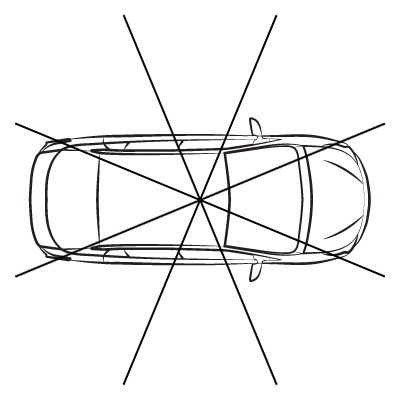
\includegraphics[width=0.3\textwidth]{car-view-8sectors}}\qquad 
   \subfigure[zwei Sektoren]{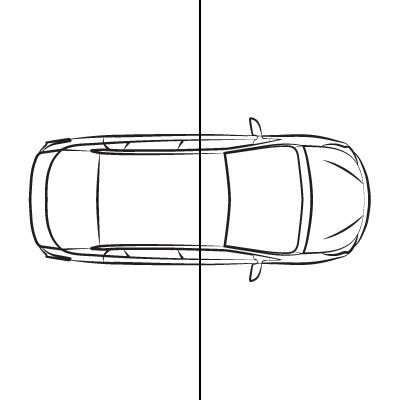
\includegraphics[width=0.3\textwidth]{car-view-2sectors}}\qquad 
   \subfigure[vier Sektoren]{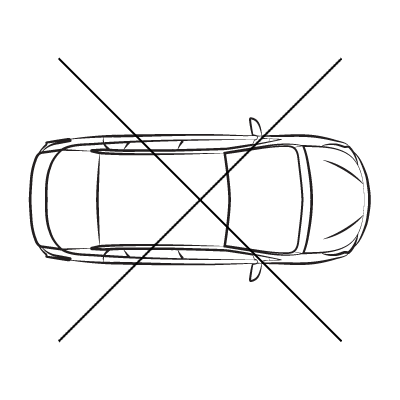
\includegraphics[width=0.3\textwidth]{car-view-4sectors}}
  \caption{mögliche Sichtfelder eines Fahrzeugs, Quelle: Auto-Silhouette vecteezy.com} 
  \label{figure:car-view-sectors}
\end{figure}

Eine solch feine Unterscheidung war nicht nötig.
Es sollte genügen, feststellen zu können, ob sich ein anderes Fahrzeug relativ zu \enquote{Ego} im vorwärtigen oder rückwärtigen Raum befindet. 
Die Abdeckung sollte ohne Unterbrechung sein.
Für die Simulation nach dem Einspurmodell von Nagel-Schreckenberg funktionierte dies ohne Probleme.
Bei einem Testlauf des Mehrspurmodells mit vier Fahrzeugen kam es zur Kollision zweier Fahrzeuge. 
Bei der anschließenden Kontrolle stellte sich heraus, dass ein Fahrzeug (vehicle0), welches sich auf der Überholspur (lane 2) befand, ein anderes Fahrzeug (vehicle20) direkt neben sich nicht \enquote*{sah} und daraufhin, so wie es der Plan vorsah, zum nächsten Schritt in die Hauptspur fährt. 
Im nachfolgenden Zeitschritt kam es dann zur Kollision.

\begin{verbatim}
--- step 365 ----------------
         vehicle20   in lane   1   in cell   333.0   @   74.21582362319865   kph
         vehicle2   in lane   1   in cell   282.0   @   129.99324819683062   kph
         vehicle0   in lane   2   in cell   333.0   @   99.94723620551235   kph
PIA1     vehicle0   sees no traffic at all -> Pull-in
         vehicle1   in lane   1   in cell   90.0   @   130.8321253026147   kph
--- step 366 ----------------
         vehicle20   in lane   1   in cell   4.0   @   74.21582362319865   kph
         vehicle2   in lane   1   in cell   289.0   @   131.11124225593747   kph
         vehicle0   in lane   1   in cell   3.0   @   100.80986539456516   kph
TFC100   vehicle0   has vehicle in-front of -> decelerate
COS      vehicle0   STOPPED -> collision
OUT      vehicle0   -> Pull-out attempt successful
         vehicle1   in lane   1   in cell   97.0   @   130.64144521630223   kph
\end{verbatim}

Das Sichtfeld der Fahrzeuge wurde zu einem Vier-Sektoren-Modell abgewandelt und die Pläne für Ein- und Ausscheren, der hiervon gleichermaßen betroffen sein dürfte, angepasst.
Es werden nun jeweils die beiden Sektoren, die die Bewegungs- bzw.Orientierungsrichtung darstellen, kontrolliert.